\subsection{Grundlagen von Bilanzräumen}

\subsubsection{Definition von Bilanzräumen}
Energiebilanzräume stellen ein zentrales Konzept im Energiemanagement dar und bilden die Grundlage für die Berechnung von Energieleistungskennzahlen, da sie deren Vergleichbarkeit sicherstellen [\cite[Kapitel 5.4.2]{Engelmann.2015}]. 
Sie umfassen laut Engelmann (2015) sowohl Energiequellen als auch Energiesenken und müssen anhand einheitlicher Kriterien definiert werden müssen. Des Weiteren besteht die Möglichkeit, 
Bilanzräume in mehrere Teilbilanzräume zu unterteilen [\cite[Kapitel 5.4.2]{Engelmann.2015}].

% TODO: Praxisbeispiel Bilanzraumzerlegung mit ableitung von Methodischen Ansätzen + breitere Quellen


\subsubsection{Bilanzierung}
Bilanzräume haben unter anderem eine Relevanz für die Bilanzierung in Organisationen. Eine Bilanzierung bezeichnet in diesem Kontext die Berechnung der in einen Bilanzraum ein- und austretenden 
Energieflüsse [\cite[S. 65]{Rönsch.2015}]. Nach der Definition von Engelmann (2015, Kapitel 5.4.2) muss dabei die Summe der Energiequellen und -senken eine Null-Bilanz ergeben. Im Rahmen des Energiemanagements steht 
die Energiebilanz im Fokus. Die Energiebilanzierung ist laut Rönsch (2015, S. 66) eine Form der Bilanzierung die auf dem Prinzip der Energieerhaltung beruht, welcher besagt, dass die Energie in einem abgeschlossenen System, über die Zeit 
konstant ist. Abgeschlossen meint in diesem Kontext wärmeundurchlässig. Für abgeschlossene Systeme ohne Speicherkapazitäten bedeutet das dass die Summe der Energiequellen gleich der Summe der Energiesenken ist, 
sollte das System über Energiespeicherkapazitäten verfügen so ist die Menge der gespeicherten Energie gleich der Differenz aus der Summe der Energiequellen und -senken [\cite{Rönsch.2015}]. 

Die Energiebilanz nach Rönsch (2015) lässt sich mathematisch mit der folgenden Gleichung darstellen:

\[
E_{\text{gespeichert}} = \sum E_{\text{quelle}} - \sum E_{\text{senke}}
\]

\textbf{Erläuterung der Gleichung:}
\begin{itemize}
    \item \(E_{\text{gespeichert}}\): Energie, die im System gespeichert wird.
    \item \(\sum E_{\text{quelle}}\): Summierte zugeführten Energie, der Energiequellen.
    \item \(\sum E_{\text{senke}}\): Summe aller Energiesenken, also der verbrauchten Energie.
\end{itemize}

Für abgeschlossene Systeme ohne Energiespeicher  gilt:
\[
E_{\text{gespeichert}} = 0
\]
In diesem Fall ist die zugeführte Energie gleich der verbrauchten Energie:
\[
\sum E_{\text{quelle}} = \sum E_{\text{senke}}
\]

%TODO: Praxisbeispiel mit Anwendung der Gleichung


\subsubsection{Energiequellen und -senken}


Die definition von Bilanzräumen mit den zu bilanzierenden Energiequellen und -senken kann grundlegend für den Aufbau eines Energieflussmodells verwendet werden. 
Ein Energieflussmodell berechnet die Massen- und Energiebilanzen sowie die thermodynamischen Gleichgewichtsbedingungen der Komponenten [\cite{FrancescaPalazzi.2007}] und stellt somit eine zentrale Komponente 
zur Energeiebilanzierung in Organisationen.


\subsubsection{Beziehungen zwischen Bilanzräumen}


\subsubsection{Praktische Herausforderung im Zusammenhang mit Bilanzräumen}
Die Definition von Bilanzräumen, wie sie von Engelmann (2015, Kapitel 5.4.2) beschrieben wird, bildet eine wesentliche Grundlage für die Analyse und Optimierung der energiebezogenen Leistung von Organisationen. 
Dabei müssen die Bilanzraumkriterien den spezifischen Gegebenheiten der Organisation angepasst werden. Dies wird deutlich, wenn man den Energieverbrauch in verschiedenen Sektoren betrachtet.

\begin{figure}[H]
    \centering
    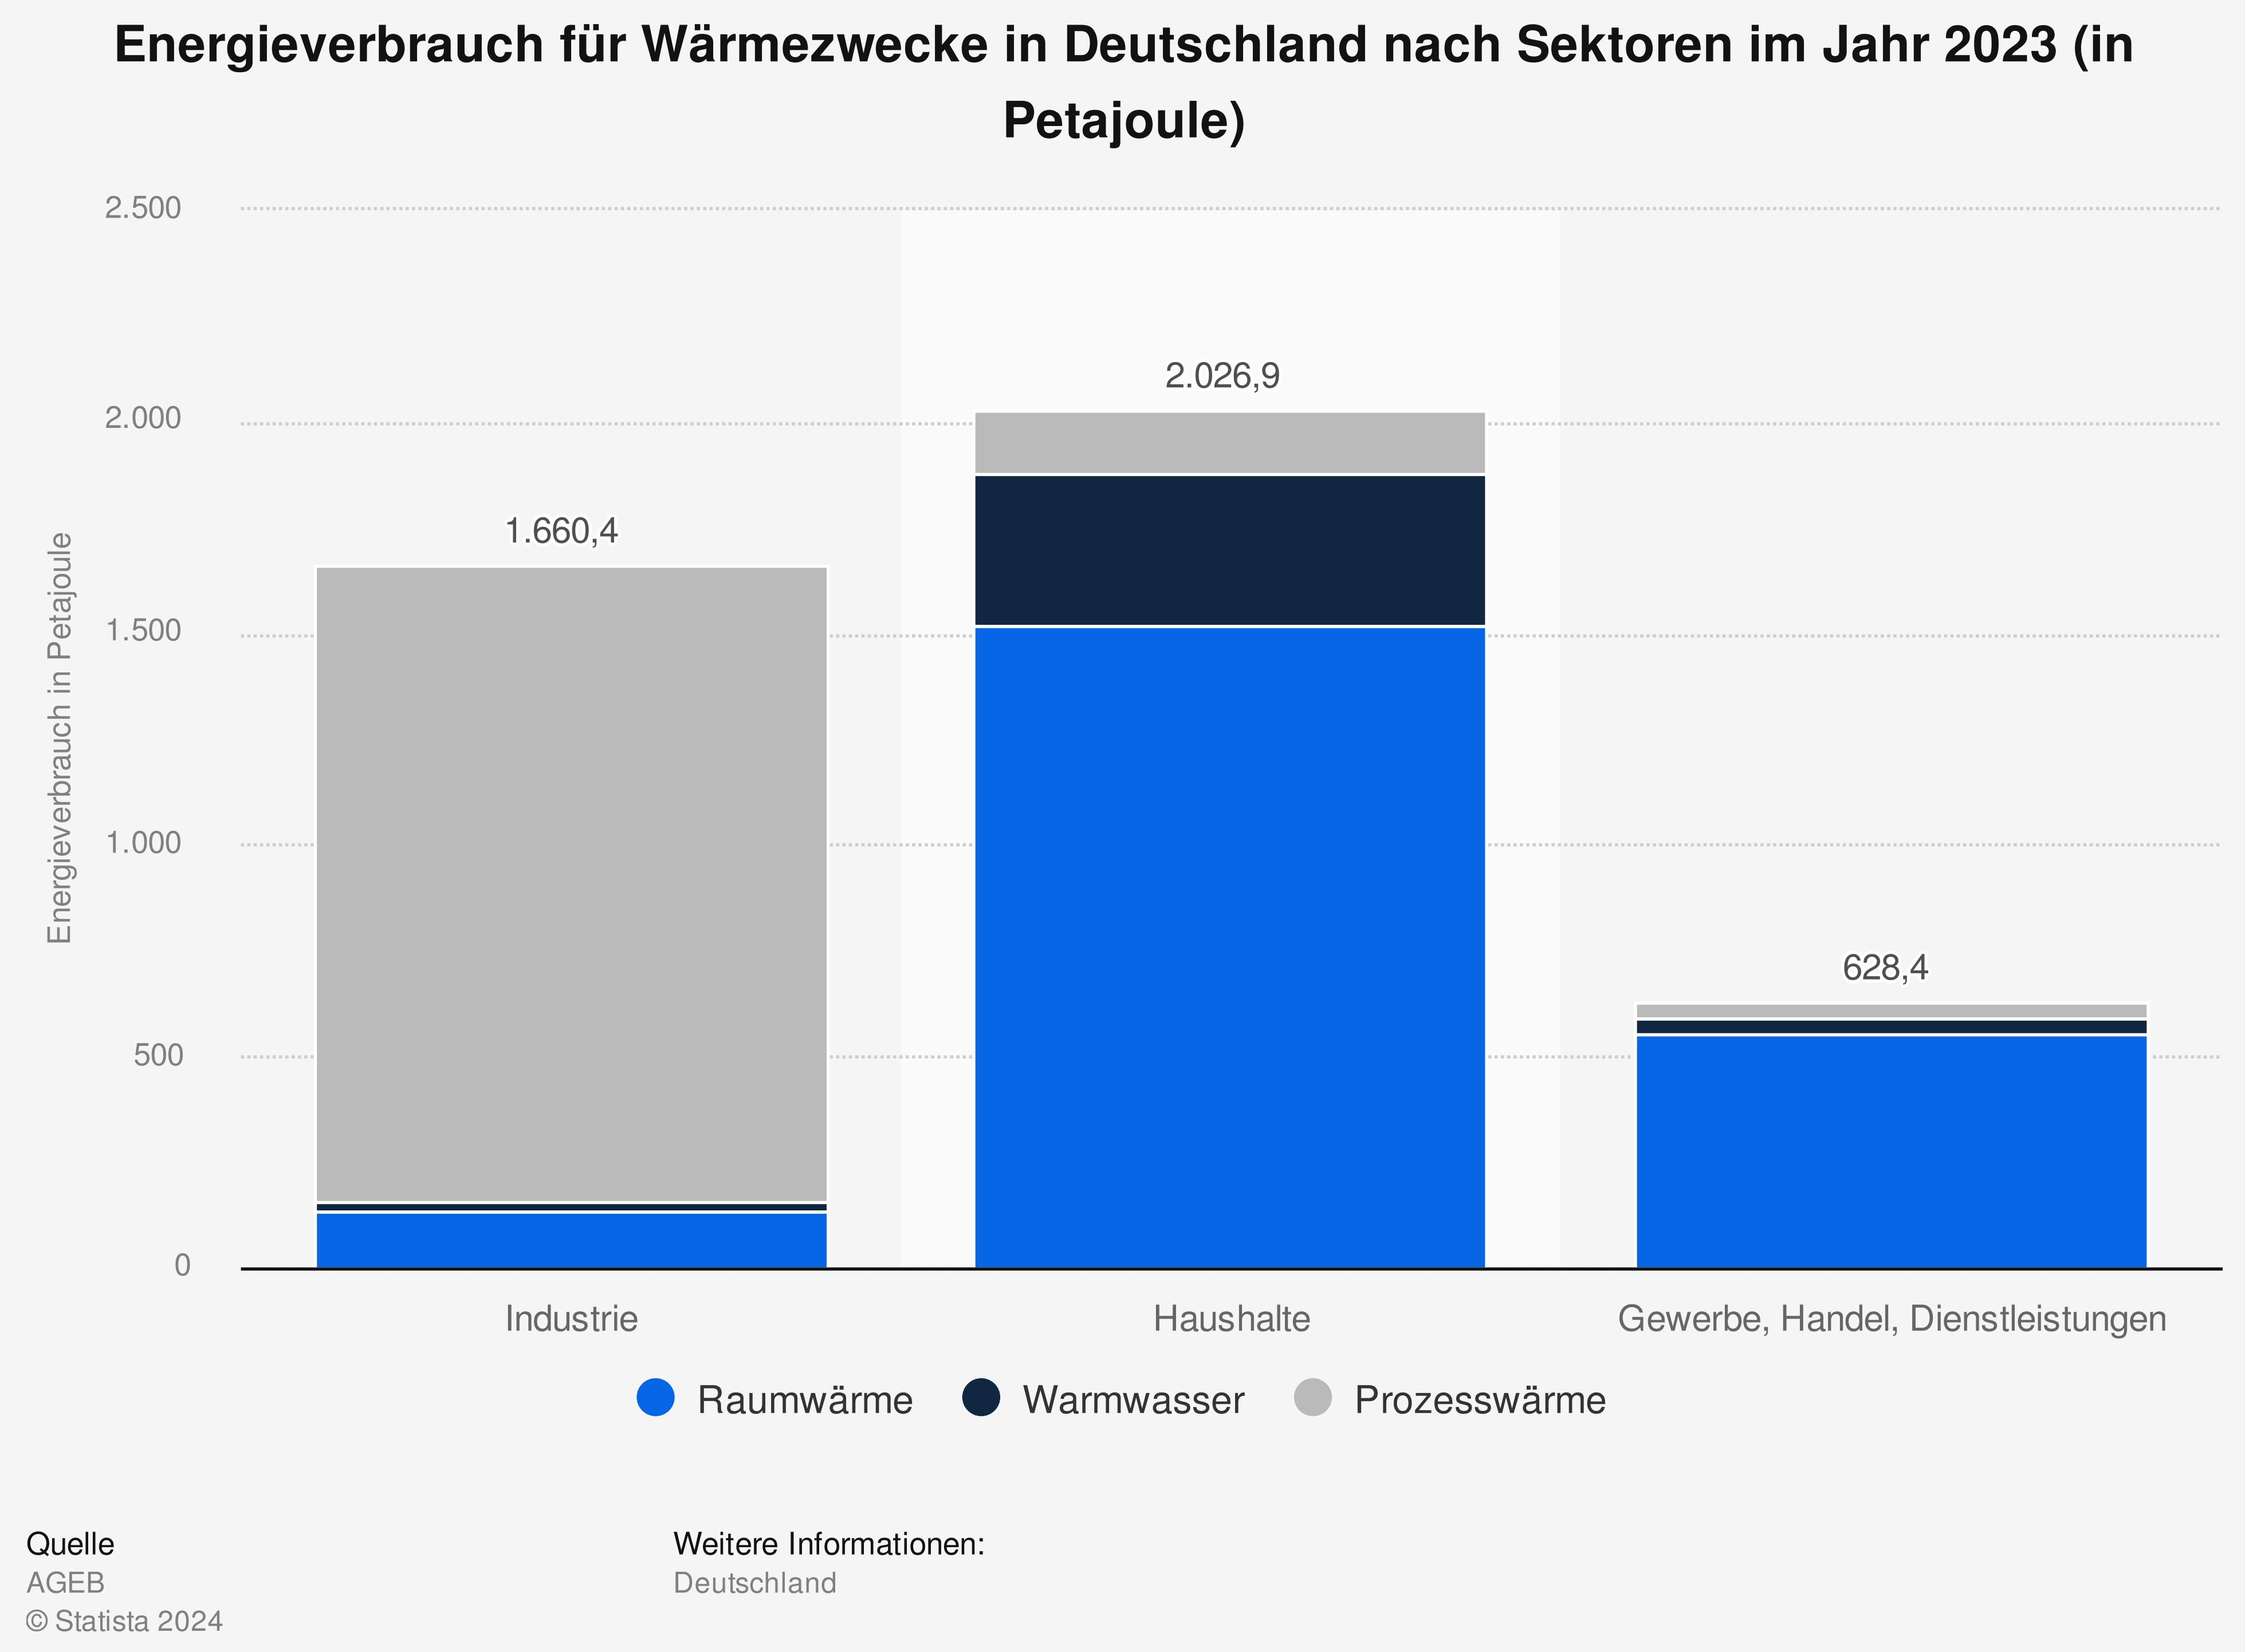
\includegraphics[width=1\textwidth]{../../Ressourcen/Bilder/Energieverbrauch_für_Wärmezweck_DE.jpg}
    \caption{Energieverbrauch für den Wärmezweck in Deutschland [\cite{AGEB.2024}]}
    \label{fig:Energieverbrauch_Wärme_DE}
\end{figure}

Abbildung \ref{fig:Energieverbrauch_Wärme_DE} zeigt den Energieverbrauch für Wärmezwecke in Deutschland im Jahr 2023, aufgeschlüsselt nach Sektoren. Hieraus lassen sich grundlegende Erkenntnisse für die 
praktische Definition von Bilanzräumen ableiten. Der industrielle Sektor weist einen hohen Anteil an prozessbezogener Wärme auf, was darauf hinweist, dass hier spezifische Bilanzräume für die Erfassung und 
Optimierung von Prozesswärme sinnvoll sind. Im Gegensatz dazu spielt im Dienstleistungssektor die Raumwärme eine dominierende Rolle denn in Organisationen, die immaterielle Dienstleistungen 
erbringen, spielt die Gebäudeenergie eine entscheidende Rolle bei der Verbesserung der energiebezogenen Leistung, während Prozesse oder Technologien eine untergeordnete Bedeutung haben [\cite{AlbertoFichera.2020}]. 
Dies erfordert andere Schwerpunkte bei der Definition von Bilanzraumkriterien.

Dieser Unterschied zeigt, dass ein einheitlicher Ansatz zur Definition von Bilanzraumkriterien sektorenübergreifend nicht zielführend ist. Stattdessen sollten die Bilanzraumkriterien auf den jeweiligen Energieeinsatz 
abgestimmt werden, um Optimierungspotenziale gezielt identifizieren zu können. Für Organisationen, die Dienstleistungen anbieten, bedeutet dies beispielsweise, dass die Gebäudeenergie als zentrale Energiesenke 
in den Fokus rückt, während bei Industriebetrieben die Energieflüsse innerhalb der Produktionsprozesse detaillierter bilanziert werden sollten.

%Ausblick: welche Relevanz haben Interdepenzen von Energiequellen und - Senken 
